\documentclass[prl,aps,superscriptaddress,twocolumn,10pt,nolongbibliography]{revtex4-2}
\usepackage[pdftex]{graphicx}
\usepackage{color}
\usepackage{amsmath,amsthm,amssymb,mathtools}
\usepackage[colorlinks=true,allcolors=blue]{hyperref}
\usepackage{enumerate}
\usepackage{sidecap}
\sidecaptionvpos{figure}{c}
\usepackage{soul}

% for inline codes
\usepackage{listings}
\usepackage{color}
\definecolor{codegreen}{rgb}{0,0.6,0}
\definecolor{codegray}{rgb}{0.5,0.5,0.5}
\definecolor{codepurple}{rgb}{0.58,0,0.82}
\definecolor{backcolour}{rgb}{0.95,0.95,0.92}
\lstdefinestyle{mystyle}{
    backgroundcolor=\color{backcolour},
    commentstyle=\color{codegreen},
    keywordstyle=\color{magenta},
    numberstyle=\tiny\color{codegray},
    stringstyle=\color{codepurple},
    basicstyle=\footnotesize,
    breakatwhitespace=false,
    breaklines=true,
    captionpos=b,
    keepspaces=true,
    numbers=left,
    numbersep=5pt,
    showspaces=false,
    showstringspaces=false,
    showtabs=false,
    tabsize=2
}
\lstset{style=mystyle}

\newcommand{\notes}[1]{\textbf{\textcolor[rgb]{1,0,0.5}{#1}}}
\newcommand{\mick}[1]{\textbf{\textcolor[rgb]{0,0.6,0.3}{#1}}}

\begin{document}
\title{CS 412: Final Report for Microbusiness Density Forecasting}
\author{Kittithat Krongchon (krongch2)}
\affiliation{Department of Physics, University of Illinois at Urbana-Champaign}
\author{Ting Cheng (tingc4)}
\affiliation{Gies College of Business, University of Illinois at Urbana-Champaign}
\date{\today}

\maketitle

% Briefly introduce your task in the selected challenge. What is the input and what is the output?
% Getting to know your data. How large is it? What is the type of your data (categorical, numerical, etc)? 
% Are there any network, text or image data included?
\section{Introduction}
\begin{figure}
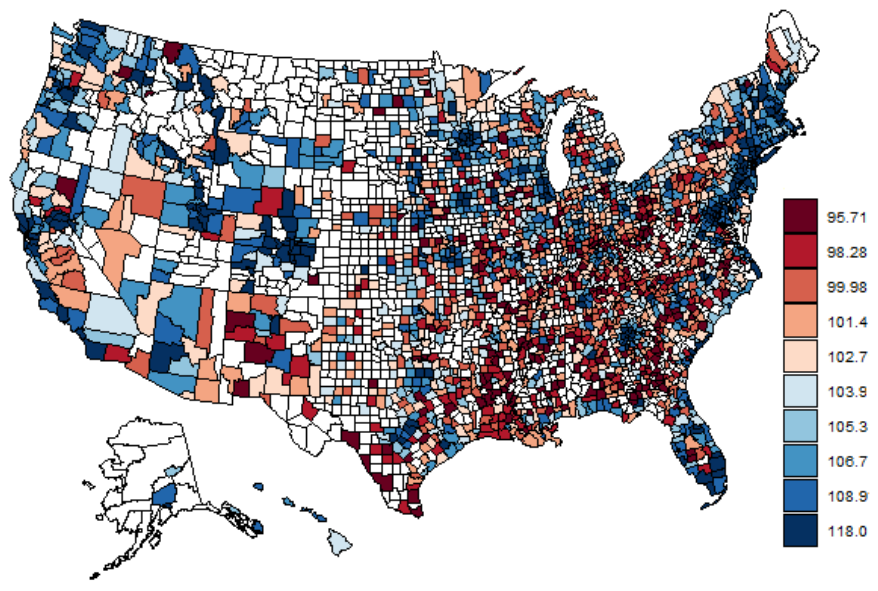
\includegraphics[width=3in]{figs/activity.png}
\caption{\label{fig:activity}
Microbusiness activity index by county in December 2021.
}
\end{figure}

Policymakers in the United States attempt to create economies that are robust to industry downturns. 
The success (or limitation) of new policies heavily relies on the data of business entities. 
Gaining accurate visibility into enabling economic decisions, however, is a challenging task because a large number of ``microbusinesses'', defined as businesses with ten or fewer employees, are often too small or too new to be included in standard data sources.
To overcome this challenge, the Venture Forward team at GoDaddy has studied tens of millions of microbusinesses in the United States for several years and has made the survey data publicly available. 
Thus, using data science techniques will enable policy leaders to gain more insights, which will be helpful for microbusiness entrepreneurs. 
This competition serves as a platform for participants to broaden the vision on the economic impact. 

\section{Data Interpretation}
The task for this competition is to forecast microbusiness activity (Fig.~\ref{fig:activity}) across the United States, as measured by the density of microbusinesses for each of the 3142 counties~\cite{yu2021godaddy}.
The values for this column are provided on a monthly basis, starting from August 1, 2019 to October 1, 2022. 
The participants are predicting the microbusiness density for the next month. 
Thus, the total number of given records is $3142 \times 41 = 128822$ rows of data.
The other columns that are provided include the percentage of households in the county with access to broadband of any type, the percent of the population in the county over age 25 with a 4-year college degree, the percent of the population in the county born outside of the United States, the percent of the workforce in the county employed in information related industries, and the median household income in the county. 
These extra columns serve as features in training models.
The total size of these datasets is 10.93MB and all of them are numerical data without unstructured data. 

In this proposal, we will explore several training approaches, most of which can be put into two classes, namely auto-regressive models and tree-based models. 

% How do you plan to solve it? Explain your idea at a high-level. (You may revise it or even propose a completely new one later. We just need to know that you have already spent some time thinking about it.)
% List at least 2 baseline approaches you would like to compare with. Add citations if they are from research papers.
\section{Method}

\subsection{Linear regression}
Even though time-series forecasting is a challenging problem and requires procedures, whose performance relies on intensive feature engineering and complex models, in the first step of this report, a simple linear regression is used to obtain a baseline of our prediction. 
Despite being one of the most common techniques to understand linear relationships between dependent variables and independent variables, the formalism for simple linear regression is included for completion. 
The model is given by 
\begin{align}
y_i = \beta_0 + \beta_1 x_{i1} + \beta_2 x_{i2} + \cdots + \beta_p x_{ip} + \epsilon_i, 
\end{align}
where $y$ represents the dependent variable, and $x_p$'s represent independent variables. 
The index i denotes the sample, and p labels the feature variables. The goal of linear regression is to find a set of $\beta$'s that can minimize the cost function given by 
\begin{align}
\frac{1}{n} \sum_i (y_{i} - \hat{y}_{i})^2.
\end{align}

This technique, however, is based on a few assumptions that affect the accuracy of the linear model~\cite{hayashi2011econometrics}. 
First, linearity is assumed because the model equation only depends on the first polynomial order of independent variables. 
For a higher order relationship, polynomial regression might be required although such a technique could result in overfitting. 
Another assumption is that the errors, $\epsilon_i$, are assumed to be independent and normal. 
The reason is given by the central limit theorem, which says the sum of a large number of independent and identically distributed random variables approaches a normal distribution. 
Since the errors represent the combined influence of one or more independent variables that are not included in the linear model, we want them to satisfy the condition for the central limit theorem. 

\subsection{Auto-regressive models}
For a time-series data, the auto-regressive integrated moving average (ARIMA) model is a widely used model that is based on constructing a model that depends on values at a different time. 
This type of model depends on the values of variables in the past, which is given by 
\begin{align}
y_t - \alpha_1 y_{t-1} &\cdots - \alpha_p y_{t-p} \nonumber \\
&= \epsilon_t + \theta_1 \epsilon_{t-1} + \cdots + \theta_q \epsilon_{t-q},
\end{align}
where $p$ and $q$ denote the order of time lags of the data (called the autoregressive model) and errors (the moving-average model). 
This model can be generalized to include the multiplicity of the roots as given by 
\begin{align}
(1 - \sum_i^p \alpha_i L^i) (1 - L)^d y_t = (1 + \sum_i^q \theta_i L^i) \epsilon_t, \label{eq:arima}
\end{align}
where $L$ is the lag operator, which moves the data by one unit of time, and $d$ is the multiplicity. 
We solve this model by looping through different combinations of $(p, d, q)$ to find the model that yields the lowest Akaike information criterion (AIC) value. 
In our analysis, the model called seasonal-ARIMAX (SARIMAX) is used, which is an extension to the ARIMA model to capture seasonal data.

\subsection{Tree-based models}
\begin{figure}
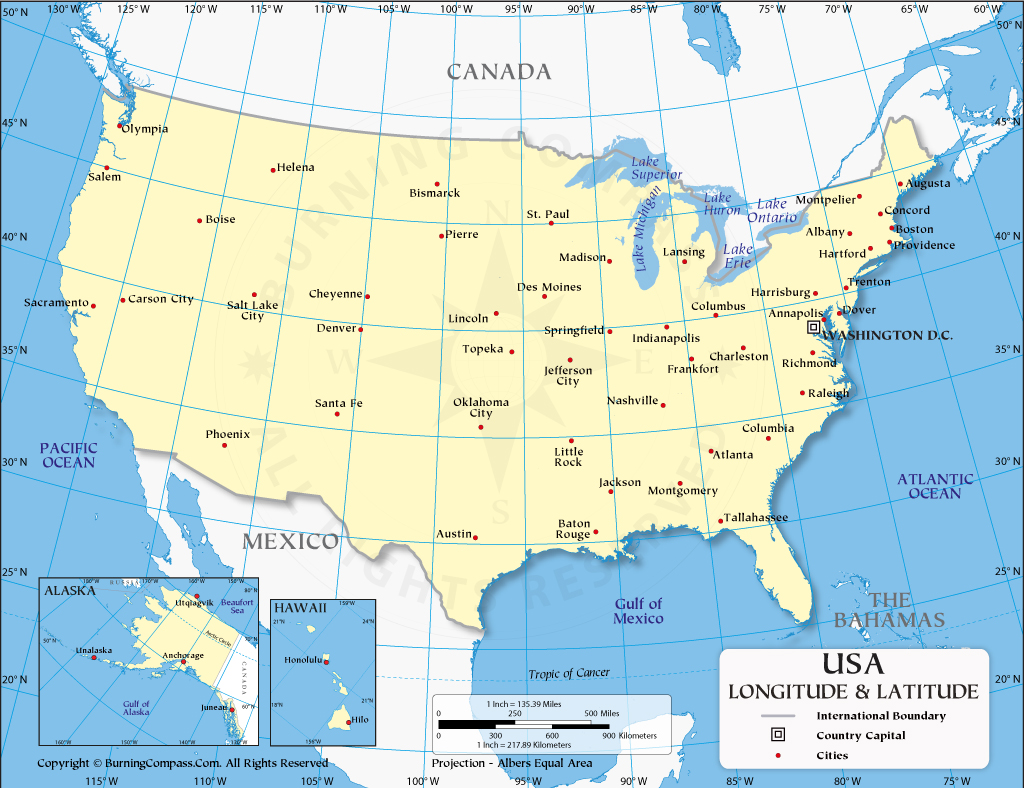
\includegraphics[width=3in]{figs/geomap.jpg}
\caption{\label{fig:geomap}
US longitude and latitude map with cities.
}
\end{figure}

Another class of techniques to be explored is tree-based models, such as random forest and XGBoost~\cite{chen2016xgboost}.
Random forest is a prediction algorithm, which is an extension of a decision tree. 
The algorithm works as follows. First, we perform a random selection with replacement on the data, i.e. bootstrapping. 
Then, we generate a decision tree on a randomly selected subset of feature variables. 
Once all the decision trees (hence forest) are obtained, we use them to predict the dependent variable from a given sample set of feature variables.

Another commonly-used method to used in regression or classification problems is gradient boosting due to improved performance over random forest~\cite{piryonesi2020data,hastie2009elements}.
The underlying principle of gradient boosting is rather similar to random forest. 
However, in random forest the trees are to be aggregated exactly as they are generated. 
Meanwhile, in gradient boosting, each tree (in this case a weak learner) is updated in such based on the so-called pseudo-residuals
\begin{align}
r_{im} &= -\frac{\partial L(y_i, F(x_i))}{\partial F(x_i)},
\end{align}
where $r_{im}$ represents the residual of the $i$-th element at the $m$-th iteration, $F(x_i)$ is a model that is trained using the data set $\{x_i, y_i\}$.
The loss function $L(y_i, F(x_i))$ is to be optimized in a one-dimensional problem to find a multiplier for the updated model.
This process is performed over several iterations to output $F_M$, which is the most recent model at the $M$-th iteration.

As the prediction is based on the different counties in the United States, we will add geographic features such as longitude and latitude as shown in Fig.~\ref{fig:geomap}~\cite{geomap}. 
This decision is based on the assumption that the counties with adjacent latitudes have similar temperature, weather, or even unemployment rates. 
The geographic features bring up hidden layers of features in tree-based models.
We use \texttt{Nominatim} from the \texttt{geopy} module to find the correlated longitude and latitude for each county in the data set.

\subsection{Evaluation}
For the evaluation of our answers, we use symmetric mean absolute percentage error (SMAPE), as given by
\begin{align}
\textrm{SMAPE} &= 100 \cdot \frac{2}{n} \sum_{i}^n \frac{|y_i - \hat{y}_i|}{|y_i| + |\hat{y}_i|},
\end{align}
where $i$ represents the month number, with the 0-th month corresponding to August 2019, $y_i$ and $\hat{y}_i$ denote the true and predicted values of microbusiness density.
While in this formula, SMAPE is undefined when both $y_i$ and $\hat{y}_i$ are zero, we avoid encountering this problem in our data by changing the target variable before training our model as discussed in the following section.

% Argue on the feasibility to finish the task on the selected challenge. 
% If your framework is too complicated, you might struggle to implement it. 
% Feel free to use existing tools and packages (e.g., repositories on GitHub).
% \section{Feasibility}
% Since the time-series prediction involved in this competition has been well explored in literature, and the existing tools are robust, this specific challenge has a straightforward workflow. 
% The challenge for us, therefore, comes down to turning the provided information into an object that is suitable for each specific tool as discussed in the previous section.

\section{Result and Discussion}

\subsection{Linear regression and ARIMA baseline models}
\begin{figure*}
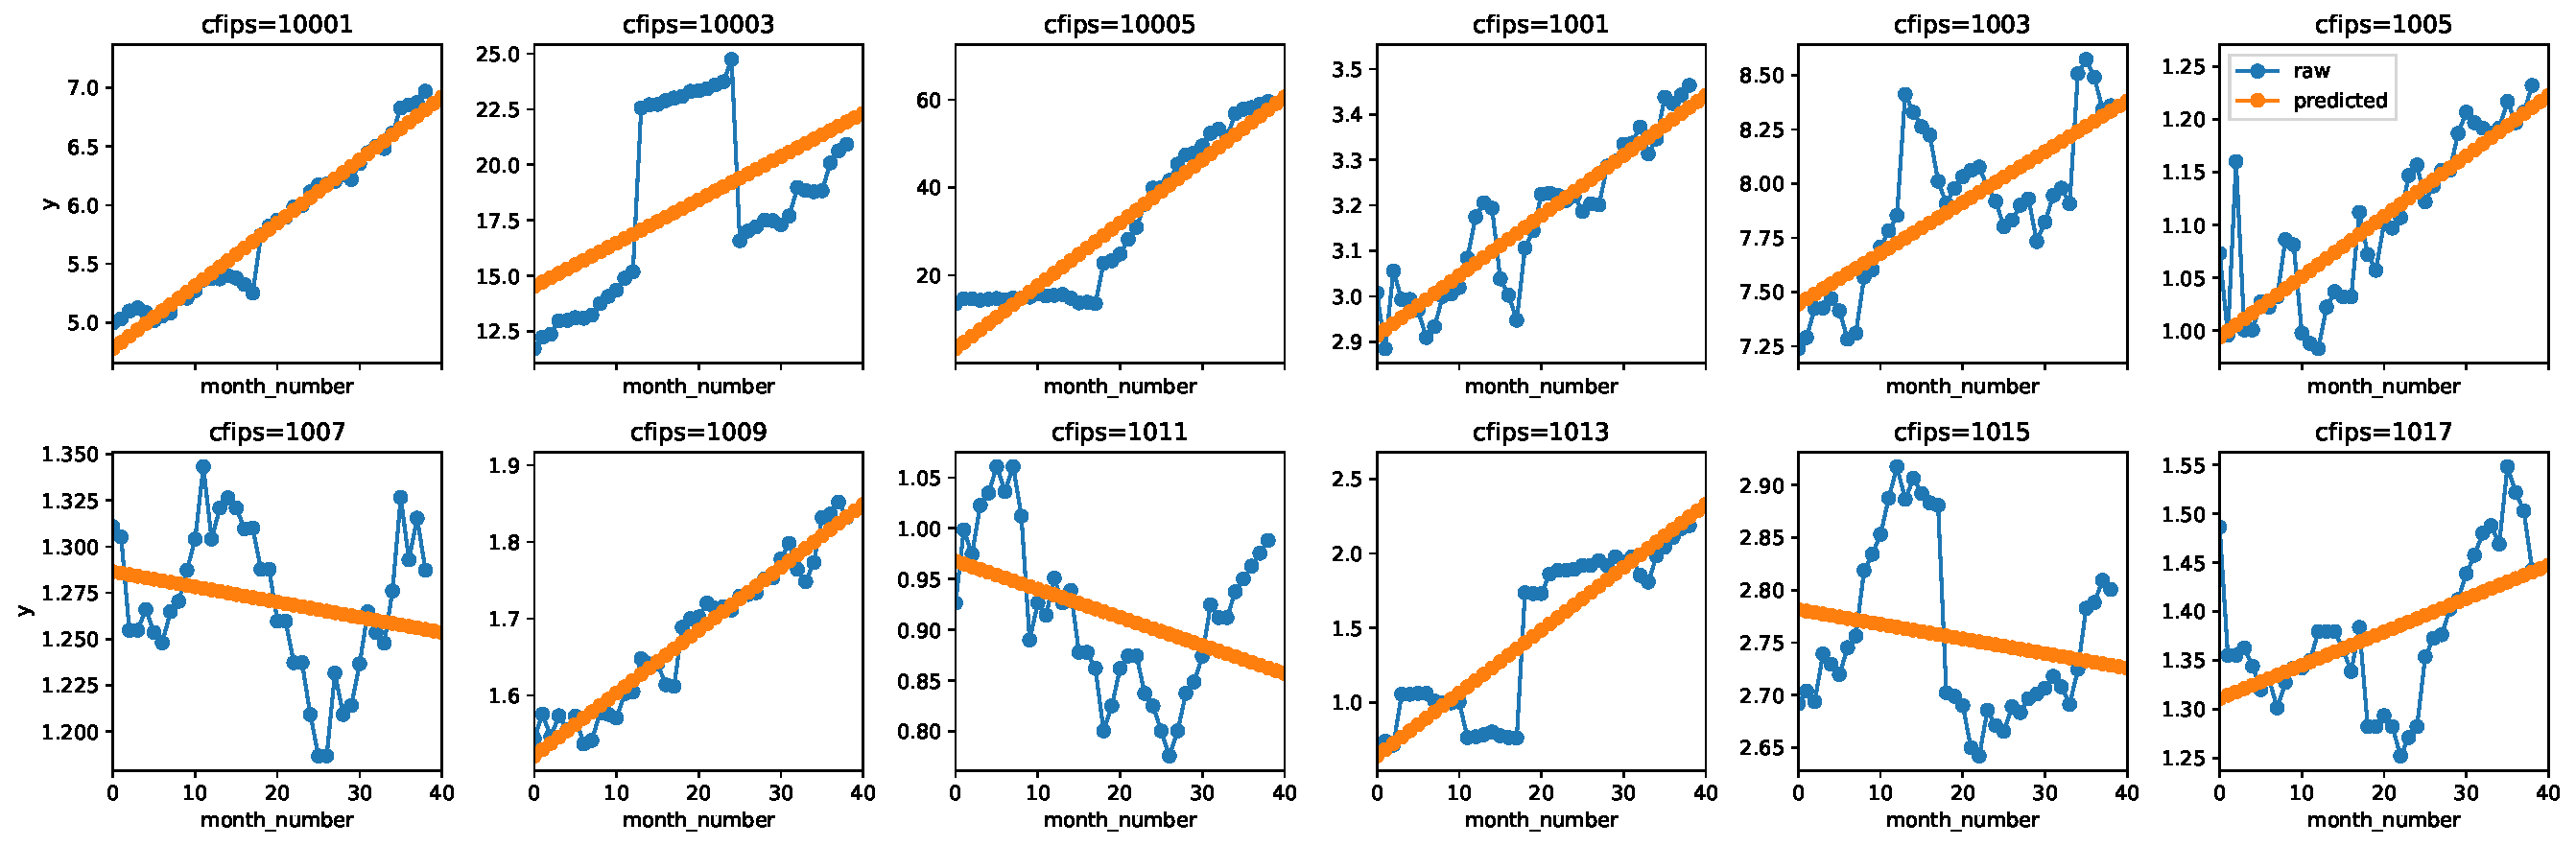
\includegraphics[width=7in]{figs/linear.pdf}
\caption{\label{fig:linear}
Linear regression: SMAPE = 8.355
}
\end{figure*}

Our implementation for the linear regression model is such that one model is used per one county, which means that there are a total of 3142 models. 
The results for some of the counties are displayed in Fig.~\ref{fig:linear}.
While the linear model can explain the raw data well for some counties, it failed to describe several counties, especially ones that have a big jump, such as CFIPS 10003 or ones that have high-amplitude fluctuations, such as CFIPS 1007 and 1011. 
Regardless of how poorly this type of models performs, this step provides us with a baseline SMAPE of 8.355, which will be improved upon.

\begin{figure*}
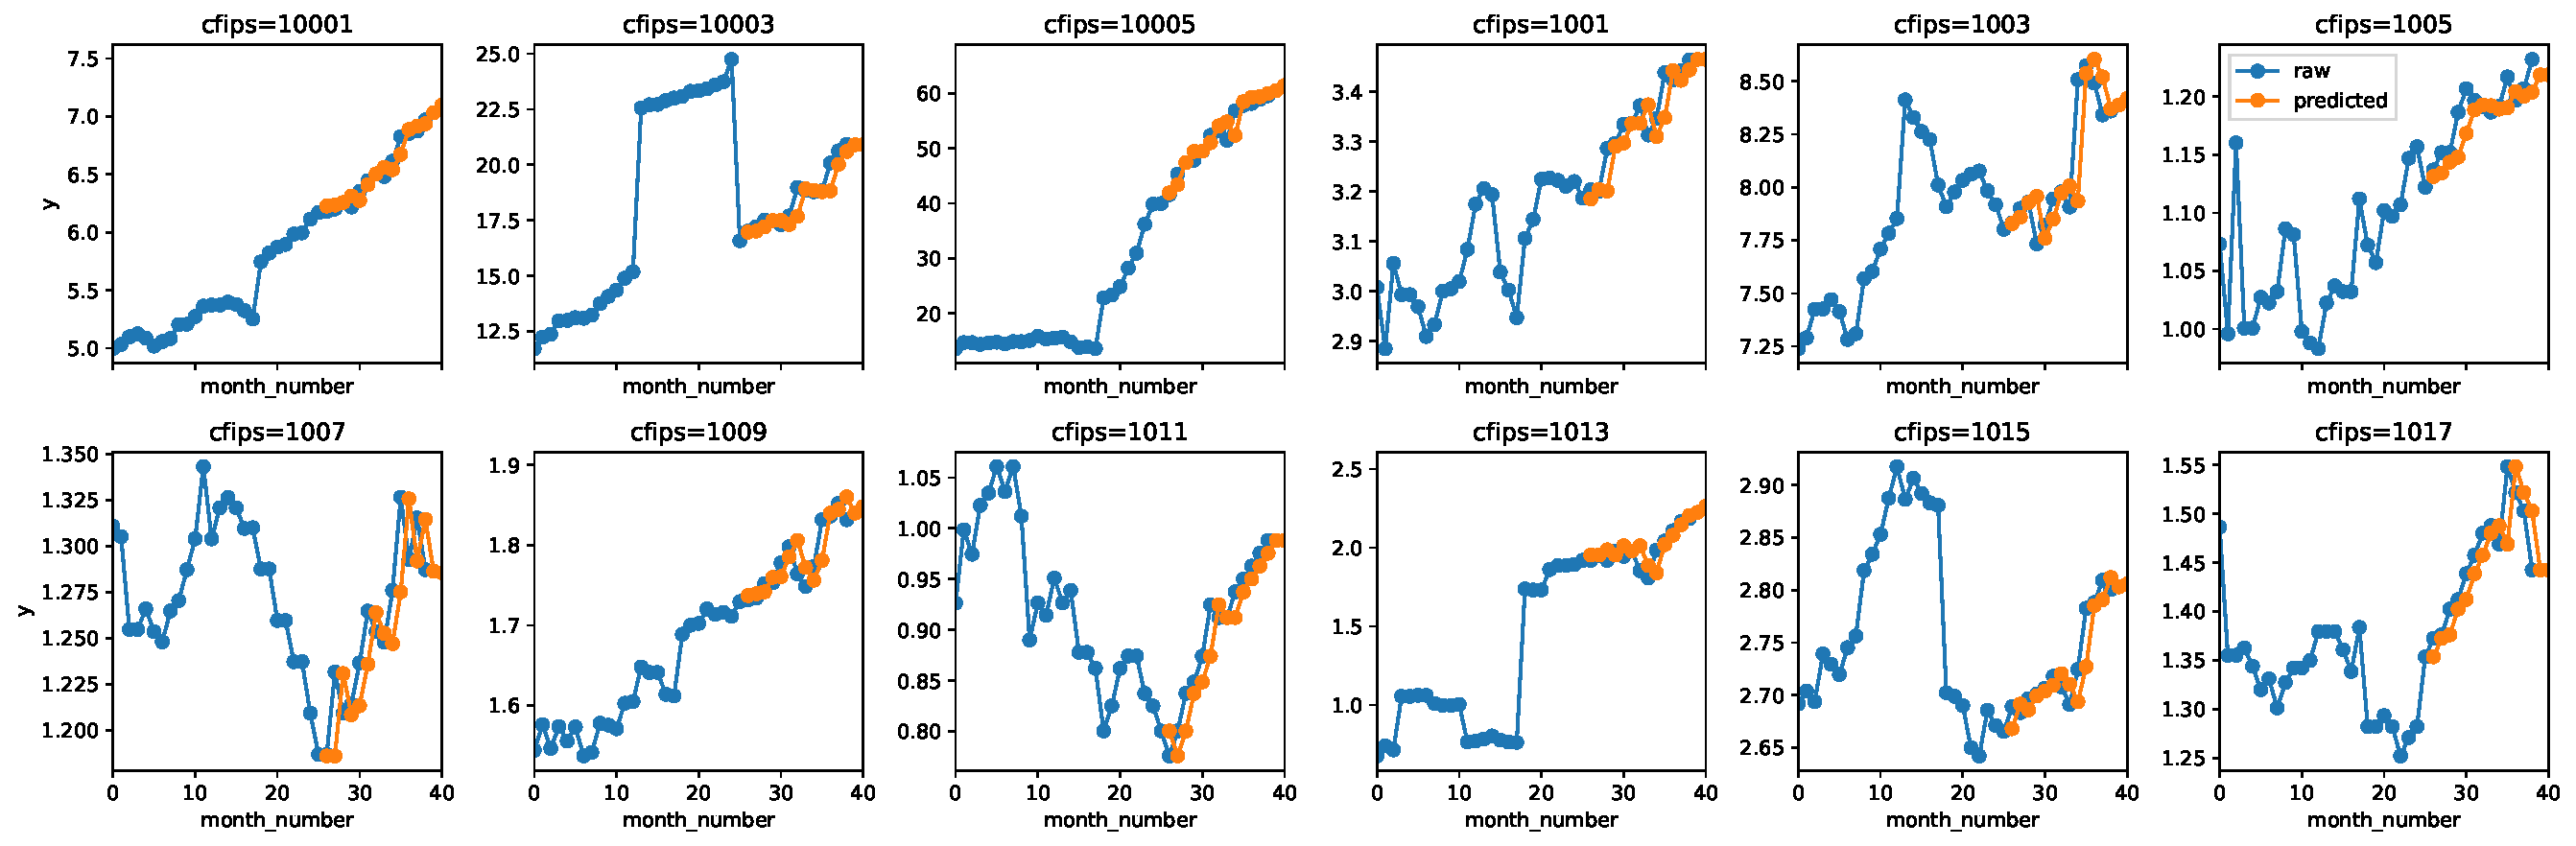
\includegraphics[width=7in]{figs/arima.pdf}
\caption{\label{fig:arima}
ARIMA: SMAPE = 4.609
}
\end{figure*}

The ARIMA implementation is similar to linear regression in the sense that each county has its own model. 
However, additional complexity is present due to the optimization process of the $(p, d, q)$ parameters as discussed in Eq.~(\ref{eq:arima}) from the Method section.
The result for ARIMA is plotted in Fig.~\ref{fig:arima}.
While this type of models results in an improvement over linear regression with SMAPE of 4.609 compared to 8.355 from before, the predicted value simply repeats the value from the previous month for each county.
This behavior means that the model does not have necessary features that would describe the data trend.
In this case, the main feature that this model learns from is the value of the previous month. 
Therefore, more features need to be included, such as geographic location or census data, which are discussed in the Timeline section.

\subsection{Gradient Boosting}
Now that we have our baseline results from linear regression and ARIMA, we are ready to move on to a more feature-dependent approach, such as gradient boosting as described in the Method section.
The hope of this approach is to generate a model that can capture the simultaneous relationship between multiple features and the microbusiness density that our baseline models have failed to do so. 
One thing to note is that this approach does not have the knowledge of time in our time-series forecasting problem. 
Therefore, many additional columns need to be created to teach the model the correlation between the past, present, and future, which results in a robust performance on time-series forecasting despite being a tree-based model~\cite{wojcik2018prognozowanie}.  

Another concern with this type of models is that it can only predict the value at time $t + 1$, where $t$ represents the month number in our case unlike linear regression or ARIMA models that can predict the value of any time given the model. 
Our solution to this problem is to use the data that has the month number between $0$ and $t$ as a training set to predict the value at time $t + 1$.
Then, we put the recently predicted data back into the training set to predict the value at time $t + 2$ and so on.
While this process might seem computationally expensive, our current problem involves predicting the microbusiness density for month 35 to month 40, which can be done within a few minutes on a laptop computer.

Our result is generated from the package \lstinline{CatBoost}~\cite{prokhorenkova2017catboost,dorogush2018catboost}, which is an extension of gradient boosting. 
This package improves GPU support, robustness on categorical features, and reducing overfitting.
The decision for choosing \lstinline{CatBoost} is based on the following reasons. 
The first reason is that our data contains categorical features, such as states and counties. 
While a technique such as one-hot encoding is normally used to handle categorical features, it creates unnecessary features, which impede the training process.
The second reason for choosing this package is that hyperparameters are the loss function can be directly specified, which allows for streamlined implementation of nested cross validation.

\subsection{Hyperparameter Tuning}
The nested cross validation is implemented to find the optimal training hyperparameters, which include learning rate, maximum bin, subsample, and maximum depth. 
The inner training sets are created by splitting the data into 6 sets, each of which corresponds to the data of 5 months. 
Thus, the overall inner training sets spans from month number 0 to month number 30.
We train each split with the with optimal hyperparameters and average each split to compare against the test sets, which are defined as the data of the next 5 months of each split.
This process, however, improves the SMAPE by roughly at most 0.3.

\subsection{Feature Engineering}
One of largest and most difficult parts of training a gradient boosting model is creating features because of the inclusion of external data.
Thus, this problem can become infinitely large as we can import multiple sources of data. 
For this report, we explore some of the basic features and later include a few sources from census and geographic location to give a sense of how well this type of model can perform.
Here, we are reporting our results on different types of features to be included and their effects on the final solution.

We start with a simple model that only the states, counties, time-series features, which are defined as follows.
We create a new column that shifts the microbusiness density value by one month, i.e. one row of data, to emulate the ability of models such as ARIMA.
We create similar columns that correspond to shifting $2, 3, \ldots, 8$ months and refer to this type of columns as ``lag'' columns.
Similarly, we create new columns that correspond to rolling mean of specified time lag to smooth out the value within a certain time frame.
We refer to this type of columns as ``rolling'' columns.
At this point, having the county, lag, and rolling features should let us obtain a result similar to that of ARIMA. 
Indeed, we find that the SMAPE from gradient boosting using such features is 4.380, which is similar to (or is even a small improvement over) the SMAPE of 4.609 from ARIMA.

Next, we add features from two sources of survey data, one from the data provided within this competition itself and the other from the annual resident population estimates published by the United States Census Bureau~\cite{uscensus}.
The first internal survey includes columns, such as the percentage of households in the county with access to broadband of any type or education as introduced in the Data Interpretation section.
The latter survey includes columns, such as total population, birth periods, death rate within periods, etc. 
Adding both of these sources results in 46 more column features, which we refer to as ``census'' columns.
The model performance after including the census columns, however, improves by only a small margin, with the SMAPE of 4.180, despite having many features. 
Thus, before we keep adding more features, it might be more productive to understand the underlying problem we are optimizing. 

The \lstinline{CatBoost} package optimizes MAPE, which is an absolute metric when fitting the model. 
However, in this competition SMAPE is used as the evaluation metric, but it is a relative metric. 
Therefore, directly predicting the microbusiness density might not be the most optimal approach because optimizing MAPE for the microbusiness density does not guarantee an optimal value for SMAPE. 
To work around this problem, we create a new column, which will be our target (not part of the features), and it is defined as the ratio between the microbusiness density at time $t-1$ divided by the value at time $t$. 
We also subtract the final value by 1 to avoid encountering zero division in SMAPE. 
Thus, the new target is given by
\begin{align}
\textrm{ratio}_t &= \frac{y_{t-1}}{y_t} - 1,   
\end{align}
where $t$ represents the month number and $y$ is the microbusiness density. 
The hope is that since this new target is a relative measurement, the optimization performance will be better reflected in the SMAPE rather than MAPE.
Thus, we will perform gradient boosting to predict the new ratio variable instead of directly predicting the microbusiness density, and we will revert the equation to retrieve microbusiness density once the training and fitting procedure is completed.
The technique results in a large improvement in the model performance with $\textrm{SMAPE} = 2.355$ for only the lag and rolling columns.
Including the census columns brings this number down to $\textrm{SMAPE} = 2.242$.

Finally, we implement the features related to geographic information. 
First, the latitude and longitude of each county is obtained from a public database~\cite{uscoordinates}. 
Then, we create features that convert the latitude and longitude into a flat coordinate as follows.
\begin{align}
x &= \cos(\textrm{latitude}) \cos(\textrm{longitude}). \\
y &= \cos(\textrm{latitude}) \sin(\textrm{longitude}). \\
z &= \sin(\textrm{latitude})
\end{align}
Training the model with these additional geographic information improves the performance even further by a small margin with $\textrm{SMAPE} = 2.156$.
We report the plot of this model in Fig.~\ref{fig:gb}. 
The SMAPE values for several multiple training schemes that we have explored are also reported in Table~\ref{tab:smape}.

\begin{figure*}
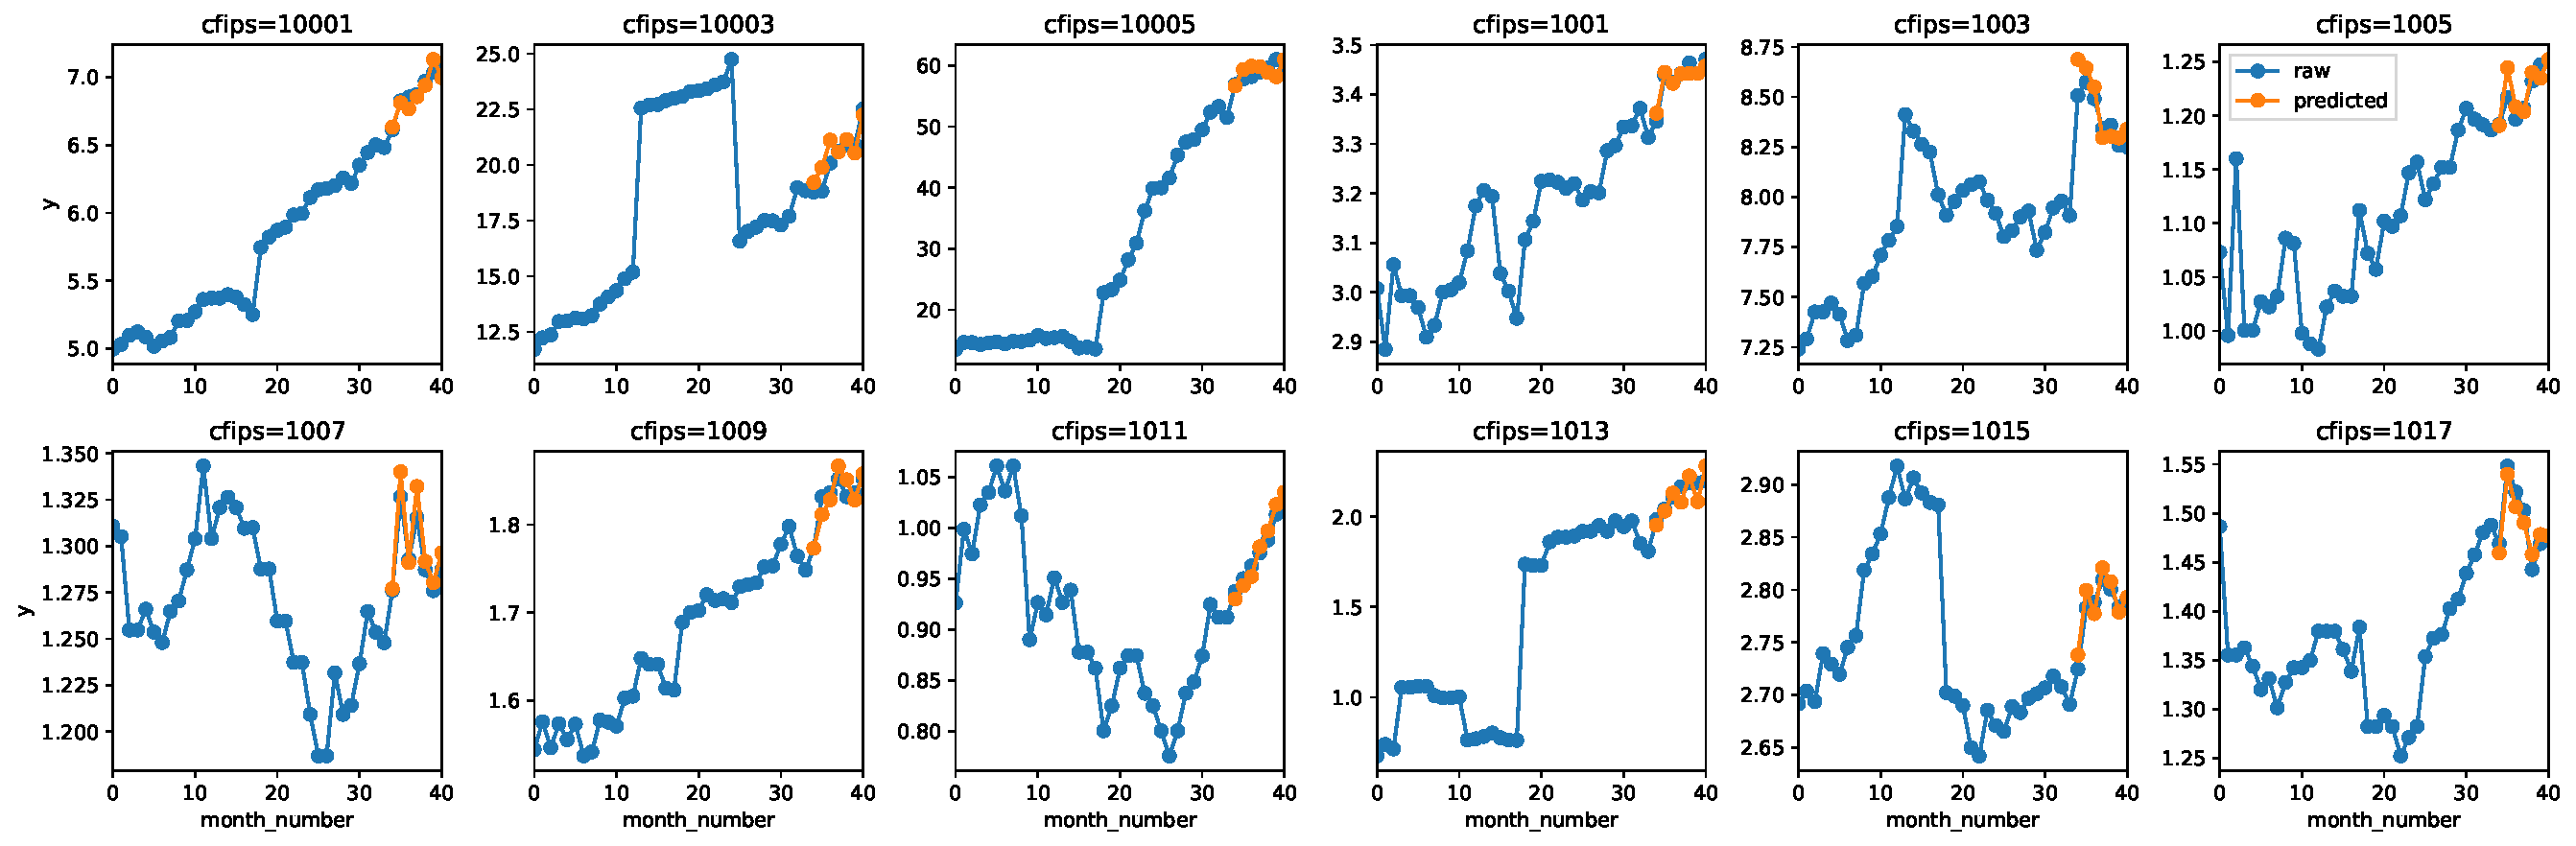
\includegraphics[width=7in]{figs/gb.pdf}
\caption{\label{fig:gb} GB(target=ratio, lag, rolling, census, geodata): SMAPE = 2.156}
\end{figure*}

\begin{table}
    \caption{
    SMAPE of multiple training schemes, including linear regression, ARIMA, and gradient boosting (GB) with several combination of features as defined in the Feature Engineering section.
    }
    \label{tab:smape}
    \begin{ruledtabular}
    \begin{tabular}{lr}
    Method and Features & SMAPE \\
    \hline
    Linear regression & 8.355 \\
    ARIMA & 4.609 \\
    GB(target=y, lag, rolling) & 4.380 \\
    GB(target=y, lag, rolling, census) & 4.180 \\
    GB(target=ratio, lag, rolling) & 2.355 \\
    GB(target=ratio, lag, rolling, census) & 2.242 \\
    GB(target=ratio, lag, rolling, census, geodata) & 2.156
\end{tabular}
\end{ruledtabular}
\end{table}

\section{Conclusion and Future Directions}
In this final report of microbusiness density forecasting, we have covered several forecasting methods, which include linear regression and ARMIA as our baseline methods.
The gradient boosting is then used as our main model while experimenting with different features. 
We find that gradient boosting with lag and rolling features is good enough to attain the performance level of ARIMA, which is to be expected because these features encode the time-series data into the model.
Adding the census columns only improves the performance a small margin. 
However, changing the target from directly predicting the microbusiness density to the time lag ratio improves the performance by almost twofold due to the ability to capture the relative nature of SMAPE.
Lastly, we have added the geographic data as our features as proposed in the early stage of this project, but the improvement is not high. 
 
There are several improvements that could be made on the implementations of our model.
First, the ARIMA model with exogenous variables was not implemented, which means that the performance of ARIMA that we have reported does not very well represent this class of technique.  
Second, hyperparameter tuning in this report was done on a relatively small grid to save computational time. Improvements could be made by expanding the parameter grid. 
Lastly, outlier analysis could be performed to eliminate uncertainties in the model prediction. For example, the anomalies near month 18 are common among several counties, which might have affected the robustness of our model. 
Overall, we are quite satisfied with the result and appreciate the insights that we have gained from this project, and we hope to expand our analysis according to the suggested directions in the future. 

% A timeline that specifies your plan to finish the course project.
\section{Timeline and Contributions}
Our analysis involves two milestones. 
First, the training of time-series data without exogenous variables using linear regression and ARIMA models has been completed.
We arrived at this stage by March 15, 2023 according to the proposed timeline.

We completed the training models using \lstinline{CatBoost} by April 15, 2023. 
Finally, the feature engineering was completed on May 1, 2023.
The tasks are distributed as follows. 
K.K. implemented nested cross validation for the time-series data to prevent overfitting and engineered features related to census data.
T.C. implemented data visualization and engineered features related to geographic location.

\bibliography{paper}{}
\end{document}
